\documentclass[11pt,a4paper]{article}

%% More layout: Get rid of indenting throughout entire document
\setlength{\parindent}{0in}
            
%Changes from Matthias Althoff and Markus Koschi:
\usepackage{array}
\usepackage{color,hyperref}
\usepackage{fancyvrb}
\usepackage{eurosym}
%\usepackage[a4paper,left=2.5cm,right=2.5cm,nohead]{geometry}
\usepackage[a4paper,margin=2.5cm]{geometry}
\usepackage{fancyhdr} %for header
\usepackage{titlesec}
\usepackage{enumitem}
\usepackage{tabularx}
\usepackage{lastpage}
\usepackage{parskip}
\usepackage{graphicx}
\usepackage{subfigure}
\usepackage{psfrag}
\usepackage{amsmath,amssymb,amsfonts}
\usepackage{mathrsfs}
\usepackage{cite}
\usepackage{pifont} %for circled numbers
\usepackage{caption}
\usepackage[amsmath,hyperref,thmmarks]{ntheorem}  %better package for proof environment
\usepackage{booktabs}
\usepackage{dirtree} % required for directory tree
\usepackage{import}
\usepackage{graphicx}
%\usepackage{caption}
\usepackage{textcomp} % for upright quotation marks
\usepackage{xspace} % for intelligent spaces


\newcommand{\sep}[1]{{\large\textbf{#1}} \vspace{0.3cm}} %seperator
\newcommand{\ra}[1]{\renewcommand{\arraystretch}{#1}} %to change the row spacing in tables
\newcommand{\brake}{\mbox{} \vspace{0cm} \mbox{}} %seperator
\newcommand{\todo}[1]{}%{\textcolor{red}{#1\xspace}} %todo (use {} if todo output should be omitted)

%\renewcommand{\sectionmark}[1]{\markright{\thesection\ #1}}

\graphicspath{{./figures/}} %Where the figures folder is located

\pagestyle{fancy} %set differnt page style for header
\fancyhead[L]{\rightmark}
\fancyhead[C]{}
\fancyhead[R]{}
\fancyfoot[L]{}
\fancyfoot[C]{\thepage}
\fancyfoot[R]{}


\fancypagestyle{firststyle}
{
   \addtolength{\headheight}{-1.05cm}
   \addtolength{\headsep}{1.05cm}
}


% % easychair.tex,v 3.4 2015/12/10
% 
% \documentclass{easychair}
% %\documentclass[EPiC]{easychair}
% %\documentclass[debug]{easychair}
% %\documentclass[verbose]{easychair}
% %\documentclass[notimes]{easychair}
% %\documentclass[withtimes]{easychair}
% %\documentclass[a4paper]{easychair}
% %\documentclass[letterpaper]{easychair}
% 
% \usepackage{doc}
% 
% % use this if you have a long article and want to create an index
% % \usepackage{makeidx}
% 
% % In order to save space or manage large tables or figures in a
% % landcape-like text, you can use the rotating and pdflscape
% % packages. Uncomment the desired from the below.
% %
% % \usepackage{rotating}
% % \usepackage{pdflscape}
% 
% % Some of our commands for this guide.
% %
% \newcommand{\easychair}{\textsf{easychair}}
% \newcommand{\miktex}{MiK{\TeX}}
% \newcommand{\texniccenter}{{\TeX}nicCenter}
% \newcommand{\makefile}{\texttt{Makefile}}
% \newcommand{\latexeditor}{LEd}
% 
% %Changes from Matthias Althoff:
% \usepackage{color,hyperref}
% \usepackage{fancyvrb}
% \usepackage{eurosym}
% \usepackage{titlesec}
% \usepackage{enumitem}
% \usepackage{tabularx}
% \usepackage{lastpage}
% \usepackage{parskip}
% \usepackage{graphicx}
% \usepackage{subfigure}
% \usepackage{psfrag}
% \usepackage{amsmath,amssymb,amsfonts}
% \usepackage{mathrsfs}
% \usepackage{cite}
% \usepackage{pifont} %for circled numbers
% \usepackage{caption}
% \usepackage{booktabs}
% %\usepackage{breakurl}

% \newtheorem{lemma}{Lemma}
% \newtheorem{definition}{Definition}[]
% \newtheorem{proposition}{Proposition}[]
\usepackage[para,online,flushleft]{threeparttable}
\DeclareMathOperator{\arccosh}{arccosh}
\DeclareMathOperator{\arcsinh}{arcsinh}
\DeclareMathOperator{\arctanh}{arctanh}
\DeclareMathOperator{\abs}{abs}
\DeclareMathOperator{\sign}{sgn}

\newcommand{\cmark}{\ding{51}}%
\newcommand{\xmark}{\ding{55}}
\renewcommand{\a}{l_f} %vehicle parameter
\renewcommand{\b}{l_r} %vehicle parameter
\newcommand{\prho}{\rho} %vehicle parameter
\newcommand{\pA}{A} %vehicle parameter
\newcommand{\sX}{\sum X} %auxiliary vehicle variable
\newcommand{\sN}{\sum N} %auxiliary vehicle variable
\newcommand{\sY}{\sum Y} %auxiliary vehicle variable
\newcommand{\sL}{\sum L} %auxiliary vehicle variable
\newcommand{\sZ}{\sum Z} %auxiliary vehicle variable
\newcommand{\sM}{\sum M} %auxiliary vehicle variable



%For XML---------------------------------------------------
\usepackage{listings}

\usepackage{color}
\definecolor{gray}{rgb}{0.4,0.4,0.4}
\definecolor{darkblue}{rgb}{0.0,0.0,0.7}
\definecolor{cyan}{rgb}{0.0,0.6,0.6}
\definecolor{darkgreen}{rgb}{0,0.5,0}

\lstset{
  basicstyle=\ttfamily,
  columns=fullflexible,
  showstringspaces=false,  
  commentstyle=\color{darkgreen}\upshape, %commentstyle=\color{gray}\upshape,
  upquote=true
}

\lstdefinelanguage{XML}
{
  morestring=[b]",
  morestring=[b]',
  %moredelim=[s][\bfseries\color{black}]{>}{<}, 
  morestring=[s]{>}{<},
  morecomment=[s]{<?}{?>},  
  morecomment=[s]{!--}{--},
  stringstyle=\color{black},
  identifierstyle=\color{darkblue},
  keywordstyle=\color{cyan},
  morekeywords={xmlns,version,ref,k,v,id,lat,lon,commonRoadVersion,benchmarkID,date,timeStepSize,author,affiliation,source,tags}% list your attributes here
}
\lstset{language=XML}
%----------------------------------------------------------


\begin{document}

\mbox{} \vspace{0.8cm} \mbox{}
\begin{center} {\Huge\textbf{CommonRoad: Documentation of the Format} \\[0.3cm] \huge(Version 2023a)} \end{center}
\vspace{0.2cm}
\begin{center} {\large Sebastian Maierhofer, Markus Koschi, Anna-Katharina Rettinger, Stefanie Manzinger, and Matthias Althoff} \\[0.2cm] Technical University of Munich, 85748 Garching, Germany
\end{center}
\vspace{0.2cm}

\noindent

\begin{abstract}
This document presents the \textit{CommonRoad} format for specifying road traffic scenarios. 
%The provided scenarios in \textit{CommonRoad} are described in the scenario documentation.
The \textit{CommonRoad} format is composed of (1) meta information about the scenario, (2) a formal representation of the road network, (3) obstacles, and (4) planning problems for the ego vehicle(s).
So far, we have not discovered any limitations when building scenarios using the proposed format.
\end{abstract}


\setcounter{tocdepth}{3}
{\small
\tableofcontents}


% !TeX root = ../CommonRoad_Format.tex

\section{Introduction}
\label{sec:introduction}
\subsection{Overview about CommonRoad}
With \textit{CommonRoad}\cite{Althoff2017a}\footnote{\href{https://commonroad.in.tum.de}{commonroad.in.tum.de}} one can store driving scenarios. The scenarios can be loaded and processed by many tools available in the CommonRoad framework, e.g., drivability-checker, route planner, motion planners.  
The scenarios can be stored in two formats which are Protocol Buffers\footnote{https://protobuf.dev/} and XML files (currently only up to version 2020a). 
In this documentation, we present the definition of CommonRoad scenarios, which are composed of (1) a formal representation of the road network (see Section~\ref{subsec:lanelets}-\ref{subsec:intersections}), (2) static and dynamic obstacles (see Section~\ref{subsec:obstacles}), and (3) the planning problem of the ego vehicle(s) (see Section~\ref{subsec:egoVehicles}). 
Additionally, all of the mentioned components consists of meta information describing the element (see Section~\ref{subsec:meta}).
%In non-collaborative scenarios, only one planning problem exists, while in collaborating scenarios several planning problems have to be solved.

A visualization of all scenarios is on our website\footnote{\href{https://commonroad.in.tum.de/scenarios/}{commonroad.in.tum.de/scenarios}}, where you can also search for specific types of scenarios.

Since CommonRoad version 2024a, the default representation of a CommonRoad scenario consists of three Protobuf files instead of a  single (Protobuf/XML) file.
However, for a better exchange of files it is possible to write and read all information in just one file.

The attribute names might vary between the different representations (XML, Protobuf, Python, C++, Matlab) to align with the corresponding naming conventions, e.g., timeStep or time\_step.


\subsection{Changes Compared to Version 2020a}

For a quick reference, we summarize the major changes of version 2024a compared to version 2020a:
\begin{itemize}
\item New intersection definition
\item Separation into three files: map, dynamic, scenario 
\item Additional elements for link to licenses and license text
\item Area for modelling parking lots, bus stops, or any other "drivable area" which is difficult to model via lanelets (concept derived from lanelet2 format)
\item Meta-information series for obstacles
\item Boundary definition separated from lanelet 
\end{itemize}



% !TeX root = ../CommonRoad_Format.tex


\section{Specification of the Format}

We designed our format such that it can represent all features, is unambiguous, and is easy to use. 
We put additional emphasis to augment the road description by its implications, i.e., our format does not just describe a traffic situation, but already provides the meaning for motion planning.
As a result, our scenarios can directly be used by a motion planner and do not require much additional computations in terms of pre-processing.
Subsequently, we describe our specification.
Note that it may differ in some cases to the data structures used in our tools, e.g., commonroad-io.

All variables are given by decimal numbers based on SI units. We use a common Cartesian coordinate frame with x-, y-, and z-axis to be able to represent all road networks including bridges and tunnels. 
If a scenario is only defined in a two-dimensional plane (which is often the case), we use the convention that all z-coordinates are zero.
Angles are measured counter-clockwise around the positive z-axis with the zero angle along the x-axis.

\colorbox{red}{Add figure for orientation since this often leads to questions.}

The overall structure of the CommonRoad format is shown by Fig.~\ref{fig:structureMap}, Fig.~\ref{fig:structureDynamic}, and Fig.~\ref{fig:structureScenario}. 
Each scenario element has a unique\footnote{Unique within the whole scenario.} ID (of type positive integer) making it possible to reference it.
The numbers in square brackets denote the number of allowed elements (while \texttt{N} can be different for each element).
%If an element is omitted (number of allowed elements is $ \geq 0$), the default value is none or its default value is specified in the description of this element.


\begin{figure}[!htpb]
	\small
	\dirtree{%
		.1 [1] commonroad\_map.
		.2 [1] map\_meta\_information.
		.2 [1] location.
		.2 [0..N] lanelets.
		.2 [0..N] stop\_lines.
		.2 [0..N] boundaries.
		.2 [0..N] areas.
		.2 [0..N] traffic\_signs.
		.2 [0..N] traffic\_lights.
		.2 [0..N] intersections.
	}
	\caption{Structure encoding map information.}
	\label{fig:structureMap}
\end{figure}

\begin{figure}[!htpb]
	\small
	\dirtree{%
		.1 [1] commonroad\_dynamic.
		.2 [1] dynamic\_meta\_information.
		.2 [1] environment.
		.2 [0..N] traffic\_light\_cycles.
		.2 [0..N] traffic\_sign\_values.
		.2 [0..N] static\_obstacles. 
		.2 [0..N] dynamic\_obstacles.
		.2 [0..N] environment\_obstacles.
		.2 [0..N] phantom\_obstacles.
	}
	\caption{Structure encoding dynamic scenario information.}
	\label{fig:structureDynamic}
\end{figure}

\begin{figure}[!htpb]
	\small
	\dirtree{%
		.1 [1] commonRoa\_scenario.
		.2 [1] scenario\_meta\_information.
		.2 [1] map\_id. 
		.2 [1] dynamic\_id.
		.2 [1..N] planning\_problems.
		.2 [0..N] coopearative\_planning\_problems.
	}
	\caption{Structure encoding scenario information.}
	\label{fig:structureScenario}
\end{figure}
\newpage % to have subsection 2.1 started after this section


\subsubsection{Benchmark ID} \label{subsec:id}
The benchmark ID of each scenarios consists of four elements: \\
\centerline{COUNTRY\_SCENE\_CONFIG\_PRED\_PROBLEM.} \\
The scenario ID has the prefix C- if the scenario has multiple planning problems, i.e. it is a cooperative planning problem (otherwise, it has no prefix).

\paragraph{COUNTRY} is the capitalized three-letter country code defined by the ISO 3166-1 standard\footnote{\url{https://www.iso.org/obp/ui/\#search/code/}}, e.g. Germany has DEU and United States has USA.
If a scenario is based on an artificial road network, we use ZAM for Zamunda\footnote{\href{https://en.wikipedia.org/?title=Zamunda&redirect=no}{en.wikipedia.org/?title=Zamunda}}.

\paragraph{SCENE} = MAP-$\{1$-$9\}^*$ specifies the road network. MAP is for rural scenarios a two/three letter city code (e.g. Muc) and for highways/major roads the road code (e.g. A9 or Lanker). It is appended by an integer counting up. Note that if COUNTRY\_SCENE is the same for two scenarios, all their lanelets are identical.

\paragraph{CONFIG} = $\{1$-$9\}^*$ specifies the initial configuration of obstacles and the planning problem(s). Note that CONFIG is counting independently for non-cooperative scenarios (i.e. only one planning problem) and cooperative scenarios (i.e. multiple planning problems), since the prefix allows to distinguish between them. Thus, if PREFIX-COUNTRY\_SCENE\_CONFIG is the same for two scenarios, the road network, initial configuration of obstacles, and the planning problem(s) are equal, and only the prediction of the obstacles differs.

\paragraph{PRED} = $\{$S,T,P$\}$-$\{1$-$9\}^*$ specifies the future behavior of the obstacles, i.e. their prediction, where S = set-based occupancies, T = single trajectories, P = probability distributions, appended by an integer to distinguish predictions on the same initial configuration but with different prediction parameters.
If no prediction is used (i.e. the scenario has no dynamic obstacles), we omit the element PRED in the benchmark ID.

\paragraph{PROBLEM} = $\{1$-$9\}^*$ ID of planning problem set.

\paragraph{Examples:} Possible examples of a benchmark ID are: C-USA\_US101-1\_123\_T-1\_3-0, DEU\_FFB-2\_42\_S-4\_3-0-2, DEU\_Hhr-1\_1\_0-2.

\subsection{Auxiliary Elements} \label{subsec:auxiliary}

Subsequently, we introduce general auxiliary geometry elements.

\paragraph{Point}
A point is the simplest primitives and described by an x-, y-, and z-coordinate.
If the z-coordinate is zero (for all two-dimensional scenarios), we omit the z-element.
\begin{figure}[!htpb]
	\small
	\dirtree{%
		.1 point OR center.
		.2 [1] x.
		.2 [1] y.
		.2 [0..1] z.
	}
	\caption{Definition of point.}
	\label{fig:auxiliary}
\end{figure}


\paragraph{Rectangle}
The element \textit{rectangle} can be used to model rectangular obstacles, e.g., a vehicle.
It is specified by the length (longitudinal direction) and the width (lateral direction), the orientation, and a center point (reference point of a rectangle is its geometric center).
The orientation and center can be omitted if their values are zero.
\begin{figure}[!htpb]
	\small
	\dirtree{%
		.1 rectangle.
		.2 [1] length.
		.2 [1] width.
		.2 [0..1] orientation.
		.2 [0..1] center.
	}
	\caption{Definition of rectangle.}
	\label{fig:auxiliary}
\end{figure}


\paragraph{Circle}
The element \textit{circle} can be used to model circular obstacles, for example a pedestrian or a vehicle by using three circles.
A circle is defined by its radius and its center (reference point of a circle is its geometric center).
Analogously to the rectangle, the center can be omitted if all its coordinates are zero.
\begin{figure}[!htpb]
	\small
	\dirtree{%
		.1 circle.
		.2 [1] radius.
		.2 [0..1] center.
	}
	\caption{Definition of circle.}
	\label{fig:auxiliary}
\end{figure}

\paragraph{Polygon}
The element \textit{polygon} can be used to model any other two-dimensional obstacle. 
A polygon is defined by an ordered list of points, in which the first one is its reference point. 
We adhere to the convention that the polygon points are ordered clockwise.
\begin{figure}[!htpb]
	\small
	\dirtree{%
		.1 polygon.
		.2 [3..N] point.
%		.3 shape.
%		.2 [1..N] rectangle/circle/polygon.
	}
	\caption{Definition of polygon.}
	\label{fig:auxiliary}
\end{figure}

%Since the position of the nodes is specified in the global coordinate frame, the configuration of the polygon is already completely described. If a polygon is used to specify the shape of an obstacle and thus the position is not relevant, one should translate the polygon such that the first node is located at the origin.
% Since dynamic obstacles are rarely described using polygons, this is not a shortcoming of our specification.


\paragraph{Shape}
Elements of type \emph{shape} specify the dimension of an object and can contain one or more elements of the geometric primitives (i.e. rectangle, circle, or polygon). Please note that we separate the representation of the dimension and position/orientation of an object into the elements shape and position/orientation (described subsequently), respectively. Thus, the shape elements should usually use the origin as center point and an orientation of zero, unless a certain offset is desired.

\begin{figure}[!htpb]
	\small
	\dirtree{%
		.1 shape.
		.2 [1..N] rectangle/circle/polygon.
	}
	\caption{Definition of shape (group).}
	\label{fig:auxiliary}
\end{figure}

\paragraph{Positions}
The position of an object is specified by the element \emph{position} which contains either a point, rectangle, circle, polygon, or lanelet (unless for a planning problem as specified later), as shown in Fig.~\ref{fig:position}.

\begin{figure}[!htpb]
	\small
	\dirtree{%
		.1 /.
		.2 [1] position.		
		.3 [1] point\\OR.
		.3 [1..N] rectangle/circle/polygon\\OR.
		.3 [1..N] lanelet (\textrm{ref to} lanelet).
	}
	\caption{Element \textit{position}.}
	\label{fig:position}
\end{figure}

Note that if the position of an object is given as an area (i.e. not a single point), the area does not enclose the geometric shape of the object, but only models the interval of possible positions, e.g. the uncertainty of the position measurement.


\paragraph{Numeric Values}
Elements describing the state of an object, e.g. orientation or velocity, can have either an exact value or an interval of values, e.g. to specify the goal state or to include uncertainties.
%More specifically, one can specify the value \texttt{exact} or as an interval by specifying the \texttt{intervalStart} and \texttt{intervalEnd}.
For example, an \textit{orientation} element can be defined using \texttt{exact} or \texttt{intervalStart} and \texttt{intervalEnd}:

\begin{figure}[!htpb]
	\small
	\dirtree{%
			.1 /.
			.2 [1] orientation.
			.3 [1] exact\\OR.
			.3 [1] intervalStart.
			.3 [1] intervalEnd.
		}
	\caption{Element \textit{orientation}.}
	\label{fig:XML_orientation}
\end{figure}

\paragraph{Time}
All time elements are not given as numeric values, but as integers (i.e. non-negative whole numbers). Thus, the time element can specify the time stamp of an time-discrete object. Since the initial time is always $0$ and the constant time step size is given in the CommonRoad root element, the time in seconds can be directly calculated.


% !TeX root = ../CommonRoad_Format.tex


\section{CommonRoad Map}

\subsection{Location of Scenarios} \label{subsec:location}
The location element consists of (1) a GeoName-ID\footnote{\href{https://www.geonames.org/}{geonames.org}}, (2) a GPS latitude coordinate, (3) a GPS longitude coordinate, (4) an optional geometrical transformation introduced in the following subsection.
If the GeoName-ID and the GPS coordinates are unknown, e.g., in artificial road networks, the GeoName-ID is set to -999 and the values of the coordinates are set to 999.

\subsection{GeoTransformation Element}
\label{para:geo_reference}

To specify the geometrical transformation which were performed while creating the lanelets, one can add a \texttt{geoTransformation} element. This may contain two children:

\begin{enumerate}
	\item The optional \texttt{geoReference} element contains a \emph{proj-strings}\footnote{\href{https://proj.org/usage/quickstart.html}{proj.org}} describing a coordinate transformation from geodetic coordinates to the projected (Cartesian) coordinates. This projection can then be used to transform the Cartesian coordinates back to geodetic coordinates used by OSM (cf. Sec.~\ref{sec:OSM}).
	\item The \texttt{additionalTransformation} element (see Fig.~\ref{fig:additionalTransformation}) describes geometrical operations which were performed (after the geoReference) to transform the Cartesian coordinates. The execution order of the transformations is according to the order of the following list:
	\begin{itemize}
		\item \texttt{xTranslation} Translating x-coordinates of all points by this value.
		\item \texttt{yTranslation} Translating y-coordinates of all points by this value.
		\item \texttt{zRotation} Rotating all points by this value around the origin, with respect to a right-handed coordinate system.
		\item \texttt{scaling} Multiplying all x- and y-coordinates by this value.
	\end{itemize}
\end{enumerate}
\begin{figure}[!htpb]
	\centering
	\begin{minipage}{7.5cm}
		\small
		\dirtree{%
			.1 /.
			.2 [0..1] additionalTransformation.
			.3 [1] xTranslation.
			.3 [1] yTranslation.
			.3 [1] zRotation.
			.3 [1] scaling.
		}
		\caption{Element \textit{additionalTransformation}}
		\label{fig:additionalTransformation}
	\end{minipage}
\end{figure}

\subsection{Lanelets} \label{subsec:lanelets}
We use {\it lanelets} \cite{Bender2014} as drivable road segments to represent the road network.
Fig.~\ref{fig:structure} shows the specification of a \textit{lanelet} element.
It is defined by its {\it left} and {\it right boundary}, where each boundary is represented by an array of points (a polyline), as shown in Fig.~\ref{lanelet1}.
Optionally, line markings (solid, dashed, broad solid, broad dashed, no line marking, unknown, where unknown is the default line marking) can be included to model the boundary more precisely.
We have chosen lanelets since they are as expressible as other formats, such as e.g. OpenDRIVE\footnote{\href{http://www.opendrive.org}{opendrive.org}}, yet have a lightweight and extensible representation.
Our converter from OpenDRIVE to Lanelets is available on our website.

A lanelet consists of the following elements:
%\begin{itemize}
%3 [1] leftBound.
%.4 [2..N] point.
%.4 [0..1] lineMarking.
%.3 [1] rightBound.
%.4 [2..N] point.
%.4 [0..1] lineMarking.
%.3 [0..N] predecessor (\textrm{ref to} lanelet).
%.3 [0..N] successor (\textrm{ref to} lanelet).
%.3 [0..1] adjacentLeft (\textrm{ref to} lanelet, \textrm{drivingDir}=same/opposite).
%.3 [0..1] adjacentRight (\textrm{ref to} lanelet, \textrm{drivingDir}=same/opposite).
%.3 [0..1] stopLine.
%.3 [1..N] laneletType: highway/urban/busStop/.../crosswalk.
%.3 [0..N] userOneWay: vehicle/car/truck/bicycle/.../pedestrian.
%.3 [0..N] userBidirectional: vehicle/car/truck/bicycle/.../pedestrian.
%.3 [0..N] trafficSignRef (\textrm{ref to} trafficSign).
%.3 [0..N] trafficLightRef (\textrm{ref to} trafficLight).
%\end{itemize}


\begin{figure}[!htpb]
	\centering
	\footnotesize
	\psfrag{a}[l][c]{lanelet (road)}
	\psfrag{b}[l][c]{lanelet (rail)}
	\psfrag{c}[l][c]{road vehicle}
	\psfrag{d}[l][c]{tram}
	\psfrag{e}[l][c]{\shortstack[l]{driving \\[-0.05cm] direction}}
	\psfrag{f}[l][c]{ego vehicle}
	\psfrag{g}[r][c]{right boundary}
	\psfrag{h}[r][c]{left boundary}
	\psfrag{i}[l][c]{\shortstack{lanelets of \\ equal length}}
	\psfrag{j}[l][c]{\shortstack{point of \\ polyline}}
	\includegraphics[width=0.9\columnwidth]{figures/stachus_uniColor_d.eps}
	\caption{Lanelets of a complex intersection in the city center of Munich. Besides roads, also tram rails are modeled by lanelets.}
	\label{lanelet1}
\end{figure}

In order to represent the graph of the road network, the elements \textit{predecessor}, \textit{successor}, \textit{adjacentLeft}, and \textit{adjacentRight} are used, which are omitted if they are empty (see Fig.~\ref{fig:structure}).
Since these elements only contain objects which are already existing, we refrain from copying their data but introduce references to the neighboring lanelets by an attribute referring to their unique ID.
The elements \textit{predecessor} and \textit{successor} can be used multiple times to represent multiple longitudinally adjacent lanelets, e.g., for a road fork.
In contrast, a lanelet can have at the most one \textit{adjacentLeft} and one \textit{adjacentRight} neighbor and thus at the most one element of this type.
The additional attribute \textit{drivingDir} specifies the driving direction of the neighboring lanelet as \texttt{same} or \texttt{opposite}.
The driving direction of a lanelet is implicitly defined by its left and right bound.

Additionally, the element \textit{stopLine} can be used to model a stop line or give way line (see Fig.~\ref{fig:stopLine}).
This element is defined by two points, representing the line.
If no points are given for a stop line, we assume that its points correspond to the end points of the lanelet it belongs to.
Optionally, traffic lights or traffic signs associated with this stop line can be specified to model the traffic conditions more precisely.
Similarly to the neighboring lanelets, traffic signs and traffic lights are already existing.
Thus, we use an attribute referring to their unique ID.
By defining the line marking (solid or dashed), a stop line or give way line can be represented.

\begin{figure}[!htpb]
	\small
	\dirtree{%
		.1 /.
		.2 stopLine.
		.3 [0..2] point.
		.3 [1] lineMarking.
		.3 [0..N] trafficSignRef (\textrm{ref to} trafficSign).
		.3 [0..N] trafficLightRef (\textrm{ref to} trafficLight).
	}
	\caption{Element \textit{stopLine}}
	\label{fig:stopLine}
\end{figure}

For precise modelling of traffic conditions, additional properties of a lanelet are required.
The element \textit{laneletType} can be used multiple times to clearly define the type of a lanelet.
In order to specify which types of traffic participants are allowed to use a lanelet and in which direction, the elements \textit{userOneWay} and \textit{userBidirectional} can be included.
The supported types and users of lanelets are listed in Tab.~\ref{tab:lanelettypeanduser}.

\begin{table}[!htb]\centering
	\caption{Types and users of lanelets.}
	\ra{1.3} 
	\begin{tabular}{@{}ll@{}} \toprule
		\textbf{LaneletType} & urban, country, highway, driveWay, mainCarriageWay, accessRamp, \\
		& exitRamp, shoulder, busLane, busStop, bicycleLane, sidewalk, crosswalk,  \\
		& interstate, intersection, unknown\\
		\textbf{User} & vehicle (car, truck, bus, motorcycle, priorityVehicle, taxi), car, truck, bus, \\ & priorityVehicle, motorcycle, bicycle, pedestrian, train, taxi\\
		\bottomrule
	\end{tabular}
	\label{tab:lanelettypeanduser}
\end{table}

Optionally, traffic signs or a traffic light valid for a lanelet can be included by referring to the unique ID of the respective element. 

%Optionally, line markings (solid, dashed, ...) or the speed limit can be included to model the traffic conditions more precisely (see Fig.~\ref{fig:XMLstructure}). Further traffic signs will be added to the \textit{CommonRoad} XML format in a later release to represent traffic conditions more precisely. %ToDo:2018b

%\begin{lstlisting}
%<lanelet id='10'>
%	<leftBound>
%		<point>
%			...
%		</point>
%		...
%		<!-- Optional -->
%		<lineMarking>solid</lineMarking>
%	</leftBound>
%	<rightBound>
%		<point>
%			...
%		</point>
%		...
%		<!-- Optional -->
%		<lineMarking>dashed</lineMarking>
%	</rightBound>
%	<predecessor ref='13'/>
%	<successor ref='17'/>
%	<adjacentLeft ref='14' drivingDir='opposite'/>
%	<adjacentRight ref='15' drivingDir='same'/>
%	<!-- Optional -->
%	<speedLimit>16.67</speedLimit>
%</lanelet>
%\end{lstlisting}

\subsubsection{Geometrical Requirements of Lanelets}

All \textit{CommonRoad} scenarios meet the following requirements, which assure that lanelets form a road without holes or incorrect overlaps.
\begin{itemize}
	\item The two polylines forming the right and left bound of a lanelet must consist of the same amount of nodes.
	In addition, the imaginary straight line connection between two corresponding nodes, one in the left and one in the right bound, should be perpendicular to the center line of the lanelet. %has to be
	\item In case of a two-lane or multi-lane road, a polyline can be shared by two lanelets, i.e. the same points are used to mark the right respectively left boundary of the corresponding lanelets.
	\item For longitudinal adjacent lanelets, the connection nodes of two consecutive lanelets have to be identical, i.e. the end nodes of the predecessor are identical to the start nodes of the successor.
	\item To ensures continuous lanes, the bounds of merging and forking lanelets start/end at the corresponding left or right bound of another lanelet, as shown in Fig.~\ref{fig:lanelets_forking_merging}.
	\begin{figure}[!htpb]
		\centering
		\resizebox{0.6\textwidth}{!}{\import{figures/}{laneletsForkingMerging.eps_tex}}
		\caption{Spatial division of merging and forking lanelets.}
		\label{fig:lanelets_forking_merging}
	\end{figure}
	\item Roads are divided in so called \textit{Lane Sections}\footnote{\href{http://opendrive.org/}{opendrive.org/}}. As shown in Fig.~\ref{fig:lane_sections}, each lane section has the same number of lateral adjacent lanelets and all lanelets start and end at the border of a lane section. Thus, all laterally adjacent lanes have the same \textit{length}, which allows us to set the lateral adjacencies correctly (e.g. in Fig.~\ref{fig:lane_sections}, lanelet 1 and 2 are lateral adjacent to each other; as well as lanelet 4, 5, and 6; and lanelet 7 and 8).
	\begin{figure}[!htpb]
		\centering
		\resizebox{0.6\textwidth}{!}{\import{figures/}{laneSection.eps_tex}}
		\caption{Definition of lane sections.}
		\label{fig:lane_sections}
	\end{figure}
\end{itemize}


\subsection{Traffic Signs} \label{subsec:traffic_signs}
The element \textit{trafficSign} is used to represent different traffic signs within the scenario (see Fig.~\ref{fig:trafficSign}). Traffic signs are always valid either from the beginning of a lanelet or the end of a lanelet. For example, a priority sign at an intersection is valid from the end of the incoming lanelet. Therefore, it is not necessary to place the sign on the lanelets which go straight, left, or right. On the other hand, a speed limit sign is valid from the beginning of a lanelet so that the speed limit has to be considered for the entire lanelet. \\
A \textit{trafficSign} element consists of one or multiple \textit{trafficSignElements}. This way, a combination of traffic signs can be represented. Additionally, the position of the traffic sign can be included and it can be specified whether the traffic sign is existent in the real world by the element \textit{virtual}, e.g., in the case one wants to add a speed limit which is in the real world outside of the captured road network. If \textit{virtual} is not specified or it is set to false, we assume that the traffic sign exists also in the real world at this position. A \textit{trafficSignElement} is defined by the \textit{trafficSignId} specified in national traffic laws and can be further described by one or multiple \textit{additionalValues}.

The currently by CommonRoad supported national traffic signs are listed in Tab.~\ref{tab:supportedNationalTrafficSigns}. In Tab.~\ref{tab:traffic_signs}, exemplary traffic signs from Germany with their description are shown.

\begin{figure}[!htpb]
	\small
	\dirtree{%
		.1 trafficSign (id).
		.2 [1..N] trafficSignElement.
		.3 [1] trafficSignID.
		.3 [0..N] additionalValue.
		.2 [0..1] position.
		.3 [1] point.
		.2 [0..1] virtual.
	}
	\caption{Element \textit{trafficSign}.}
	\label{fig:trafficSign}
\end{figure} 

\begin{table}[!htb]\centering
	\caption{Exemplary German traffic sign IDs supported by CommonRoad with the corresponding symbol.}
	\ra{1.3} 
	
	\begin{tabular}{>{\centering\arraybackslash}m{3cm} m{4cm} >{\centering\arraybackslash}m{6cm}} \toprule
		\textbf{Symbol} \footnotemark & \textbf{Description}&Traffic Sign ID \\ \midrule
		\includegraphics[scale=0.035]{{./figures/102.eps}} & Right before left rule & 102 \\
		
\includegraphics[scale=0.03]{{./figures/205.eps}} & Yield &  205\\
		
\includegraphics[scale=0.04]{{./figures/206.eps}}& Stop & 206\\
		
\includegraphics[scale=0.04]{{./figures/260.eps}} & Ban on motorcycles and multi-lane vehicles & 260 \\	
		
\includegraphics[scale=0.04]{{./figures/272.eps}} & No U-turn & 272 \\
		
\includegraphics[scale=0.04]{{./figures/274.eps}}& Speed limit & 274 \\
		
\includegraphics[scale=0.04]{{./figures/275.eps}}& Required speed & 275 \\
		
\includegraphics[scale=0.04]{{./figures/276.eps}}& No overtaking (except of non-motorized traffic participants, trains, and motorcycles without sidecar) & 276 \\
		
\includegraphics[scale=0.035]{{./figures/301.eps}} & Right of way & 301\\
		
\includegraphics[scale=0.04]{{./figures/306.eps}} & Priority road & 306\\
		
\includegraphics[scale=0.04]{{./figures/310.eps}} & Town sign & 310 \\
		
\includegraphics[scale=0.04]{{./figures/720.eps}} & Green arrow sign & 720 \\
		\bottomrule
	\end{tabular}
	\label{tab:traffic_signs}
\end{table}

\begin{table}[!htb]\centering
	\caption{Overview of all supported traffic signs. Valid for complete lanelet expresses that the traffic sign is always valid from the start of a lanelet. All traffic signs which are not mentioned in this list are valid starting starting from the end of a lanelet.}
	\ra{1.3} 
	\begin{tabular}{@{}lp{9cm}p{4cm}@{}} \toprule
		\textbf{Country} & \textbf{Traffic Sign ID} & \textbf{Valid for complete lanelet} \\ \midrule
		Germany & 101, 102, 108, 114, 123, 138, 142-10,
		201, 205, 206, 208, 209-10, \mbox{209-20}, \mbox{220-10}, \mbox{220-20}, \mbox{222-10}, \mbox{222-20} ,237, 239, 242.1, 242.2, 244.2, 
		244.2, 245, 250, 251, 253, 254, 255, \mbox{257-54}, 259, 260, 261, 262, 264, 265, 266, 26, 272, 
		274, 274.1, 274.2, 275, 276, 277, 278, 281, 282, 301, 306, 308, 310, 325.1, 
		325.2, 327, 330.1, 330.2, 331.1, 331.2, \mbox{333-21}, 333-22, 350, 357, 
		\mbox{625-10}, \mbox{625-11}, \mbox{625-12}, \mbox{625-13}, \mbox{625-20}, \mbox{625-21}, \mbox{625-22}, \mbox{625-23}, \mbox{626-10}, \mbox{626-20}, \mbox{626-30}, \mbox{626-31}, 720, 
		\mbox{1000-10}, \mbox{1000-11}, \mbox{1000-20}, \mbox{1000-21}, \mbox{1000-30}, \mbox{1000-31}, \mbox{1001-30}, \mbox{1001-31}, \mbox{1002-10}, \mbox{1002-12}, \mbox{1002-13}, 
		\mbox{1002-20}, \mbox{1002-22}, \mbox{\mbox{1002-23}, 1002-11}, \mbox{1002-14}, \mbox{1002-21}, \mbox{1002-24}, \mbox{1004-30}, \mbox{1004-31}, \mbox{1020-30}, \mbox{1022-10}, \mbox{1024-10}, \mbox{1026-36}, \mbox{1026-37}, \mbox{1026-38}, \mbox{1040-30}, \mbox{1053-33} & 
		101, 102, 108, 114, 123, 138, 142-10, 201,
		208, 209-10, 209-20, 220-10, 220-20, 222-10, 222-20, 237, 239, 242.1, 244.1, 245, 250, 251, 253, 254, 255, 257-54, 259, 260, 261, 262, 264, 265, 266, 267, 274, 274.1, 275, 276, 277,
		308, 310, 325.1, 327, 330.1, 331.1 \\
		USA & R2-1, R3-4 & R2-1 \\
		\bottomrule
	\end{tabular}
	\label{tab:supportedNationalTrafficSigns}
\end{table}


\subsection{Traffic Lights} \label{subsec:traffic_lights}
The element \textit{trafficLight} is used to represent traffic lights within the scenario (see Fig.~\ref{fig:trafficLight}). Each phase/color of a \textit{trafficLight} and its duration is defined by the element \textit{cycleElement}. Similarly to the \textit{time} elements, the duration is not given as numeric value, but as integer. The color value inactive indicates that currently no phase is activated, e.g. a green right arrow traffic light can be activated iteratively. The order of the different phases is determined by the order of the \textit{cycleElements} in the element \textit{cycle}. By specifying the element \textit{timeOffset}, the cycle is shifted by this value. 

In order to define for which driving direction the traffic light is valid, i.e., the direction arrow(s) in a traffic light, the direction can be included. If the direction is not specified, the traffic light is valid for all directions. Additionally, the element \textit{active} can be used to determine whether a traffic light is active or not. Optionally, the position of the traffic sign can be included. Traffic lights are always valid starting from the end of a lanelet. 

\begin{figure}[!htpb]
	\small
	\dirtree{%
		.1 trafficLight (id).
		.2 [1] cycle.
		.3 [1..N] cycleElement.
		.4 [1] duration.
		.4 [1] color: red/redYellow/green/yellow/inactive.
		.3 [0..1] timeOffset.
		.2 [0..1] position.
		.3 [1] point.
		.2 [0..1] direction: right/straight/left/leftStraight/straightRight/leftRight/all.
		.2 [0..1] active: true/false.
	}
	\caption{Element \textit{trafficLight}.}
	\label{fig:trafficLight}
\end{figure}

%The length of each state of the traffic light is specified by the elements \textit{red}, \textit{redYellow}, \textit{green} and \textit{yellow}.
\newpage
\subsection{Intersections}  \label{subsec:intersections}
The element \textit{intersection} is used to represent an intersection within the road network (see Fig.~\ref{fig:intersection}). An \textit{intersection} element is defined by at least one \textit{incoming}, which consist of \textit{incomingLanelets}, \textit{outgoingsRight}, \textit{outgoingsStraight}, \textit{outgoingsLeft}, the element \textit{isLeftOf}, and the element \textit{crossing}. 

The elements \textit{outgoingsRight}/\textit{Straight}/\textit{Left} are used to infer for which lanelets the traffic light is valid for and to facilitate the calculation of priorities at intersections. The element \textit{isLeftOf} is used to infer the right-before-left-rule. The element \textit{crossing} models lanelets which cross other lanelets, e.g., crosswalks. Since all elements of a \textit{incoming} are already existing, we use an attribute referring to their unique ID. An example for an \textit{intersection} with all elements except crossings is illustrated in Fig.~\ref{fig:intersection}.
\begin{figure}[!htb]
	\centering
	\footnotesize
	\psfrag{A}[l][c]{incoming}	
	\psfrag{B}[l][c]{outgoingsRight}
	\psfrag{C}[l][c]{outgoingsStraight}
	\psfrag{D}[l][c]{outgoingsLeft}
	\psfrag{E}[l][c]{isLeftOf}
	\psfrag{F}[l][c]{crossing}
	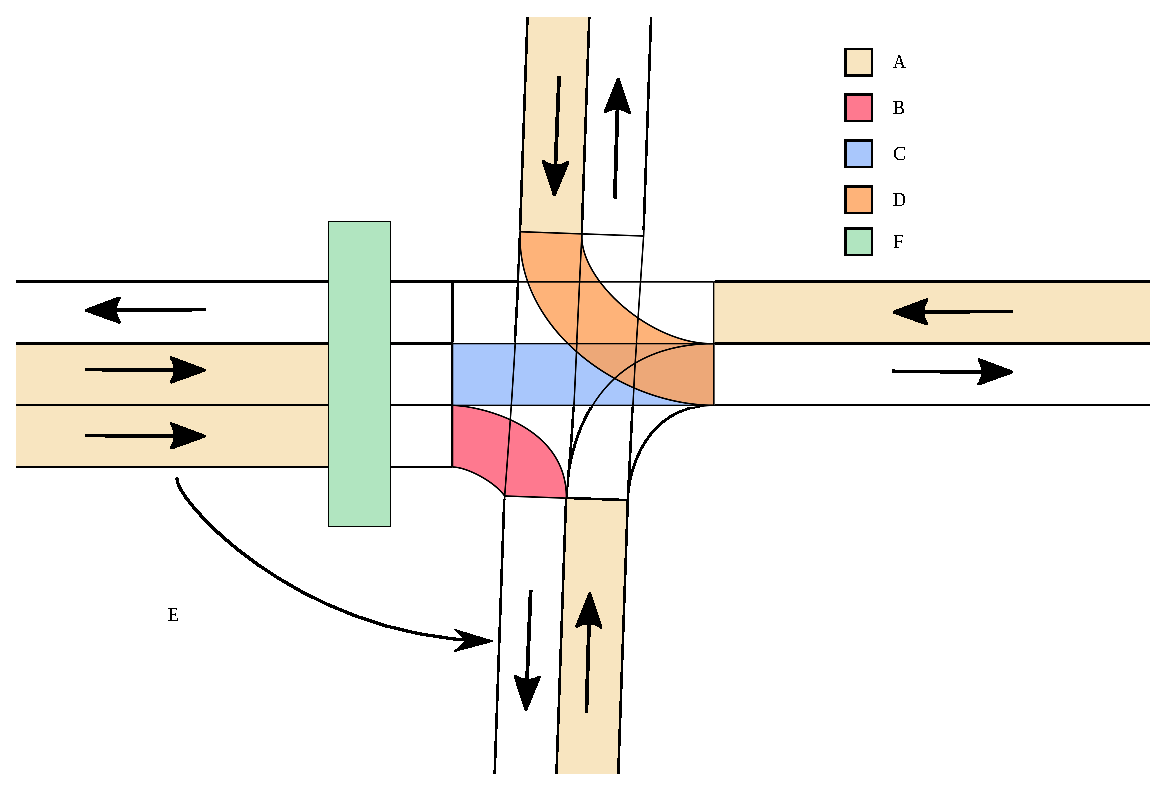
\includegraphics[width=0.6\columnwidth]{figures/intersection.eps}
	\caption{Example intersection. For better visibility, only one example lanelet is highlighted for each outgoingsRight/Straight/Left element.}
	\label{fig:intersection}
\end{figure}
\begin{figure}[!htb]
	\small
	\dirtree{%
		.1 intersection (id).
		.2 [1..N] incoming (id).
		.3 [1..N] incomingLanelet (\textrm{ref to} lanelet).
		%	.4 [0..1] stopLine.
		%	.5 [2] point.
		%	.3 [0..N] trafficSign.
		%	.3 [0..N] trafficLight.
		.3 [0..N] outgoingsRight (\textrm{ref to} all lanelets that complete the right turn within this intersection).
		.3 [0..N] outgoingsStraight (\textrm{ref to} all lanelets that are going straight).
		.3 [0..N] outgoingsLeft (\textrm{ref to} all lanelets that are turning left).
		.3 [0..1] isLeftOf (\textrm{ref to} incoming).
		.2 [0..N] crossing.
		.3 [1..N] crossingLanelet (\textrm{ref to} lanelet (usually of type crosswalk)).
		%	.3 [0..N] trafficSign.
		%	.3 [0..N] trafficLight.
	}
	\caption{Element \textit{intersection}.}
	\label{fig:intersection}
\end{figure}

\footnotetext{\href{https://commons.wikimedia.org}{commons.wikimedia.org}}


\subsubsection{Environment Obstalces}
The element \textit{environmentObstacle} is used to specify the outline of environmental or infrastructure objects to properly compute occlusions. A \textit{environmentObstacle} is specified by its type, e.g. building, and its shape. 



% !TeX root = ../CommonRoad_Format.tex

\section{CommonRoad Dynamic}
Subsequently, we specify the dynamic CommonRoad elements: dynamic obstacles, static obstacles, phantom obstacles, environment information, traffic light cycles, and dynamic traffic sign information.
Compared to the scenario format version 2020a, we separate this information from the scenario to be able to store it in a separate file for memory efficiency, e.g., one could specify several scenarios from a single dynamic information.
An overview about the structure of the dynamic element is given in \cref{fig:structureDynamic}.

\begin{figure}[!htpb]
	\small
	\dirtree{%
		.1 [1] commonroad\_dynamic.
		.2 [1] dynamic\_meta\_information.
		.2 [0..1] environment.
		.2 [0..N] traffic\_light\_cycles.
		.2 [0..N] traffic\_sign\_values.
		.2 [0..N] static\_obstacles. 
		.2 [0..N] dynamic\_obstacles.
		.2 [0..N] phantom\_obstacles.
	}
	\caption{Structure encoding dynamic scenario information.}
	\label{fig:structureDynamic}
\end{figure}

\subsection{Dynamic Meta Information}
The dynamic meta-information is identical to the scenario-meta information for which the definition can be found in \cref{sec:scenario_meta_info}.

\subsection{Environment}
The optional element \textit{environment} contains information about the time (in hours, minutes and seconds) at which the scenario starts, the time of day, the current weather, and the underground.
\begin{figure}[!htpb]
	\centering
	\begin{minipage}{10cm}
		\small
		\dirtree{%
			.1 /.
			.2 [0..1] time.
			.2 [0..1] timeOfDay: night/day.
			.2 [0..1] weather: sunny/light\_rain/heavy\_rain/fog/snow/hail.
			.2 [0..1] underground: wet/clean/dirty/damaged/snow/ice.
		}
		\caption{Structure encoding \textit{environment} information.}
		\label{fig:environment}
	\end{minipage}
\end{figure}

\subsection{Dynamic Map Elements}
Some map elements might change between real-world recordings dynamically, e.g., traffic light cycles and dynamic traffic signs.
If one would integrate them in the map directly, map sharing between scenarios is not possible.

\subsubsection{Traffic Light Cycle}
Each phase/color of a \textit{trafficLight} and its duration is defined by the element \textit{cycleElement}. 
Similarly to the \textit{time} elements, the duration is not given as numeric value, but as integer. 
The color value inactive indicates that currently no phase is activated, e.g. a green right arrow traffic light can be activated iteratively. 
The order of the different phases is determined by the order of the \textit{cycleElements} in the element \textit{cycle}. By specifying the element \textit{timeOffset}, the cycle is shifted by this value. 
The element \textit{active} can be used to determine whether a traffic light is active or not.
Each traffic light cycle references the ID of the physical traffic light it corresponds to.

\begin{figure}[!htpb]
	\small
	\dirtree{%
		.1 trafficLightCycle.
		.2 [1] trafficLightID.
		.2 [1..N] cycleElements.
		.3 [1] duration.
		.3 [1] color: red/redYellow/green/yellow/inactive.
		.2 [0..1] timeOffset.
		.2 [0..1] active: true/false.
	}
	\caption{Element \textit{trafficLight}.}
	\label{fig:trafficLight}
\end{figure}

\subsubsection{Traffic Sign Value}
Dynamic traffic signs, e.g., as they exist on German interstates, can change their sign type and value depending on the current traffic flow and weather conditions.
Therefore, we provide the option to specify a concrete sign in the dynamic information.
\begin{figure}[!htpb]
	\small
	\dirtree{%
		.1 trafficSignValue.
		.2 [1] trafficSignID.
		.2 [1..N] trafficSignElement.
	}
	\caption{Element \textit{trafficSignValue}.}
	\label{fig:trafficSign}
\end{figure} 

The definition of a \textit{trafficSignElement} can be found in \cref{fig:trafficSignElement}.


\subsection{Dynamic Obstacles}
Each dynamic obstacle element can have a \textit{type}, where we currently support the following types: \textit{car, truck, bus, motorcycle, bicycle, pedestrian, priorityVehicle, train, phantom, unknown}.
The structure of a dynamic obstacle is shown in \cref{fig:dynamicObstacle}.
Please note that only elements of either of the following three behavior models may be present: with known behavior, with unknown behavior, or with unknown stochastic behavior. 
We do not use these different behavior models together for dynamic obstacles within one traffic scenario.
Dynamic obstacle can also contain additional meta information for each time step and an ID to an obstacle from another dateset.
This information might be helpful when working with CommonRoad scenarios created from external datasets.

\begin{figure}[!htpb]
	\small
	\dirtree{%
		.1 dynamicObstacle \quad (with either of the three future behaviors).
		.2 [1] obstacleID.
		.2 [1] type: car/truck/.../unknown.
		.2 [1] shape.
		.2 [1] initialState.
		.2 [0..1] trajectory \quad \# dynamic with known behavior.
		.3 [1..N] state \\\hspace*{-0.5cm}OR.
		.2 [0..1] occupancySet \quad \# dynamic with unknown behavior.
		.3 [1..N] occupancy\\\hspace*{-0.5cm}OR.
		.2 [0..1] probabilityDistribution \quad \# dynamic with unknown stochastic behavior.
		.2 [0..1] initialSignalState. 
		.2 [0..1] signalSeries.
		.3 [1..N] signalState.
		.2 [0..1] initialMetaInformationState. 
		.2 [0..1] metaInformationSeries.
		.3 [1..N] metaInformationState.
		.2 [0..1] externalDatasetID.
	}
	\caption{Structure of a dynamicObstacle.}
	\label{fig:dynamicObstacle}
\end{figure}

The dimensions of an obstacle is specified by the element \textit{shape} (cf. \cref{subsec:auxiliary}), and its initial configuration by the element \textit{initialState}. 
Additionally, the element \textit{initialSignalState} and \textit{initialMetaInformationState} can be included, to account for properties which are not related to the movement of an obstacle, e.g., whether the indicators are turned on or off or metrics like the safe distance to the preceding vehicle.

\paragraph{Initial state}
The configuration of an obstacle at the initial time ($ t = 0$) is specified by the element \textit{initialState} with the following state variables: \textit{position}, \textit{orientation}, \textit{time}, \textit{velocity} (scalar),  \textit{acceleration} (scalar), \textit{yawRate}, and \textit{slipAngle}, as shown in Fig.~\ref{fig:initialState}. 

\begin{figure}[!htpb]
	\small
	\dirtree{%
		.1 /.
		.2 initialState.
		.3 [1] position.		
		.3 [1] orientation.
		.3 [1] time.
		.4 [1] exact.
		.5 [1] $0$.
		.3 [0..1] velocity.
		.3 [0..1] acceleration.
		.3 [0..1] yawRate.
		.3 [0..1] slipAngle.
		%		.3 [0..1] curvature.
		%		.3 [0..1] curvatureChange.
	}
	\caption{Element \textit{initialState} of an obstacle, where each state variable (except time) can be exact or an interval.}
	\label{fig:initialState}
\end{figure}


\subsection{Dynamic Obstacles with Known Behavior}
A dynamic obstacle with known behavior contains a trajectory of states a series of signals, and meta-information series (cf. \cref{fig:dynamicObstacle}). 
The trajectory allows us to represent the states of a dynamic traffic participant along a path for $t > 0$. 
The signal series allows to model non-physical properties of a dynamic obstacle, e.g. horn or lights for $t > 0$.

\paragraph{States}
The time-discrete states of a trajectory are specified by the element \textit{state}, e.g., with the following state variables: \textit{position}, \textit{orientation}, and \textit{time}, \textit{velocity} (scalar),  \textit{acceleration} (scalar), \textit{yawRate}, and \textit{slipAngle}, as shown in Fig.~\ref{fig:state}. 
The available states are based on the CommonRoad vehicle-models.
The CommonRoad vehicle-model documentation contains all available state elements.
%Note that we optionally include acceleration as a state variable for obstacles to provide additional information, e.g. for motion prediction, even though acceleration is often used as input for vehicle models.


\begin{figure}[!htpb]
	\small
	\dirtree{%
		.1 /.
		.2 state.
		.3 [1] time.
		.3 [1] position.
		.3 [1] orientation.
		.3 [0..1] velocity.
		.3 [0..1] acceleration.
		.3 [0..1] yawRate.
		.3 [0..1] slipAngle.
	}
	\caption{Element \textit{state} of a trajectory, where each state variable can be exact or an interval.}
	\label{fig:state}
\end{figure}

\paragraph{Signal Series State}
The time-discrete states of a signal series are specified by the element \textit{signalState} with the following state variables: \textit{time}, \textit{horn}, \textit{indicatorLeft}, \textit{indicatorRight},  \textit{brakingLights}, \textit{hazardWarningLights}, and \textit{flashingBlueLights}, as shown in Fig.~\ref{fig:signalState}.
The \textit{initialSignalState} is defined as the signal series state, except that the initial time is pre-defined ($ t = 0$) as for normal states.

\begin{figure}[!htpb]
	\small
	\dirtree{%
		.1 /.
		.2 signalState.
		.3 [1] time.
		.3 [0..1] horn.
		.3 [0..1] indicatorLeft.
		.3 [0..1] indicatorRight.
		.3 [0..1] brakingLights.
		.3 [0..1] hazardWarningLights.
		.3 [0..1] flashingBlueLights.
	}
	\caption{Element \textit{signalState} of a signal series.}
	\label{fig:signalState}
\end{figure}

\paragraph{Meta Information Series State}
The time-discrete states of a meta information series are specified by the element \textit{metaInformationState} (cf. \cref{fig:metaInformationState}).
Since the meta data might be different for each scenario, i.e., name and type of the meta-data, we define it as dictionaries (aka maps) for the data types string, boolean, float, and int, where the name of the data is the key. 
The \textit{initialMetaInformationState} is defined as the meta information series state, except that the initial time is pre-defined ($ t = 0$) as for normal and signal series states.

\begin{figure}[!htpb]
	\small
	\dirtree{%
		.1 metaInformationState.
		.2 [1] time.
		.2 [1] metaDataStr \quad \# map<string, string>.
		.2 [1] metaDataInt \quad \# map<string, int>.
		.2 [1] metaDataFloat \quad \# map<string, float>.
		.2 [1] metaDataBool \quad \# map<string, bool>.
	}
	\caption{Element \textit{metaInformationState} of a meta information series.}
	\label{fig:metaInformationState}
\end{figure}


\subsubsection{Dynamic Obstacles with Unknown Behavior}
For motion planning, we often do not know the exact future behavior of dynamic obstacles, but we instead represent their future behavior by bounded sets. 
Thus, dynamic obstacles with a unknown behavior are specified by an \textit{occupancy set}, which represents the occupied area over time by bounded sets. 
As shown in Fig.~\ref{fig:dynamicObstacle}, an \textit{occupancy set} contains a list of \textit{occupancy} elements.


\paragraph{Occupancies}
The \textit{occupancy} element consists of a shape (occupied area) and a time, as shown in Fig.~\ref{fig:occupancy}.

\begin{figure}[!htpb]
	\small
	\dirtree{%
		.1 /.
		.2 occupancy.
		.3 [1] shape.
		.3 [1] time.
		.4 [1] exact\\OR.
		.4 [1] intervalStart.
		.4 [1] intervalEnd.		
	}
	\caption{Element \textit{occupancy} of an occupancy set.}
	\label{fig:occupancy}
\end{figure}


\subsubsection{Dynamic Obstacles with Unknown Stochastic Behavior}
One can describe unknown stochastic behavior by probability distributions of states. 
Since many different probability distributions are used, we only provide a placeholder for probability distributions. 
\todo{Note that this element needs further refinement.}
\todo{Further details will follow.} 

%\begin{lstlisting}
%<obstacle id='60'>
%	<role>dynamic</role>
%	<type>car</type>
%	<shape>
%		...
%	</shape>
%	<probabilityDistribution>
%		...
%	</probabilityDistribution>
%</obstacle>
%\end{lstlisting}

%\paragraph{Probability Distribution}
%We can either describe the occupancy by bounded regions that evolve over time or by probability distributions. We approximate the probability distribution by their level sets, where each level set is modeled by a shape (e.g. polygon) and assigned with a probability.

%\begin{lstlisting}
%<probabilityDistribution>
%	...
%</probabilityDistribution>
%\end{lstlisting}

%If we describe the occupancy as a bounded set, we use a single level set with probability 1 obtained from set-based prediction\cite{Althoff2016d}.
%\begin{lstlisting}
%<occupancy>
%	<levelSet>
%		<shape>
%			...
%		</shape>
%		<probability>1</probability>
%	</levelSet>
%	<time>
%		...
%	</time>
%</occupancy>
%\end{lstlisting}

\subsection{Static Obstacles}
A static obstacle has no further information, as shown in \cref{fig:staticObstacle}.
Static obstacles are only placed temporarily somewhere and cannot move without external influences, e.g., a car or a building are no static obstacles but a road cone would be a static obstacle.
The shape and initial state are defined as for dynamic obstacles.
We support the following types for static obstacles: pillar, road cone, ...

\begin{figure}[!htpb]
	\small
	\dirtree{%
		.1 staticObstacle.
		.2 [1] type: pillar/.../unknown.
		.2 [1] shape.
		.2 [1] initialState.
	}
	\caption{Element \textit{staticObstacle}.}
	\label{fig:staticObstacle}
\end{figure} 

\subsection{Phantom Obstalces}
The element \textit{phantomObstacle} is used to specify potential occluded obstacles. 
They are not specified by a trajectory, but an occupancy set, similar as dynamic obstacles with unknown behavior.
They do not have an initial state.
The initial state is included in the occupancy set.


\begin{figure}[!htpb]
	\small
	\dirtree{%
		.1 phantomObstacle.
		.2 [1] phantomObstacleID.
		.2 [1] occupancySet.
		.3 [1..N] occupancy.
	}
	\caption{Element \textit{phantomObstacle}.}
	\label{fig:phantomObstacle}
\end{figure} 


% !TeX root = ../CommonRoad_Format.tex

\section{CommonRoad Scenario}






\subsubsection{Tags for Scenarios} \label{subsubsec:tags}

To allow users to select scenarios meeting their needs, the list of scenarios on our website can be filtered by the tags given in the element \texttt{tags}.  %We currently support the following list of tags: $\mathtt{urban}$, $\mathtt{highway}$, $\mathtt{race\_track}$, $\mathtt{rural}$, $\mathtt{lane\_following}$, $\mathtt{lane\_change}$, $\mathtt{turn\_left}$, $\mathtt{turn\_right}$, $\mathtt{u\_turn}$, $\mathtt{comfort}$,  $\mathtt{evasive}$, $\mathtt{lane\_blocked}$, $\mathtt{traffic\_jam}$, $\mathtt{no\_oncoming\_traffic}$, $\mathtt{roundabout}$, $\mathtt{intersection}$,  $\mathtt{oncoming\_traffic}$, $\mathtt{cut\_in}$, $\mathtt{illegal\_cut\_in}$,  $\mathtt{ghost\_driving}$, \\ $\mathtt{single\_lane}$, $\mathtt{two\_lane}$, $\mathtt{multi\_lane}$, $\mathtt{parallel\_lanes}$,  $\mathtt{mergin\_lanes}$, $\mathtt{slip\_road}$.
Additionally, the filtering based on the number of static obstacles, dynamic obstacles, obstacle types, type of future behavior of obstacles, number of ego vehicles, number of goal states, and time horizon of the scenario is possible.

%\subsubsection{Type of road}
%\label{subsec:road_type}
%\begin{align*}
%\mathtt{type\_of\_road} \iff \mathtt{urban} \lor \mathtt{interstate} \lor \mathtt{race\_track} \lor \mathtt{rural} \lor ...
%\end{align*}
%
%\subsubsection{Type of required planning maneuver}
%\label{subsec:plan_maneuver_type}
%\begin{align*}
%\mathtt{required\_planning\_maneuver} \iff \mathtt{lane\_following} \lor \mathtt{lane\_change} \lor \mathtt{turn\_left} \\
%\lor \, \mathtt{turn\_right} \lor \mathtt{u\_turn} \lor \mathtt{comfort} \lor \mathtt{evaisve} \lor ...
%\end{align*}
%
%\subsubsection{Traffic regulations}
%\label{subsec:traffic_regulations}
%\begin{align*}
%\mathtt{traffic\_regulations} \iff \mathtt{speed\_limit} \lor \mathtt{no\_overtaking} \lor ...
%\end{align*}
%
%\subsubsection{Behavior of other vehicles}
%\label{subsec:behavior_other_vehicles}
%\begin{align*}
%\mathtt{behavior\_other\_vehicles} \iff \mathtt{lane\_blocked}  \lor \mathtt{traffic\_jam} \lor \mathtt{no\_oncoming\_traffic} \\
% \lor \, \mathtt{oncoming\_traffic} \lor \mathtt{cut\_in} \lor \mathtt{illegal\_cut\_in} \lor \mathtt{ghost\_driving} \lor ...
%\end{align*}
%
%\subsubsection{Road elements}
%\label{subsec:road_elements}
%\begin{align*}
%\mathtt{road\_elements} \iff \mathtt{single\_lane}  \lor \mathtt{two\_lane} \lor \mathtt{multi\_lane} \lor \mathtt{parallel\_lanes} \\
%\lor \,  \mathtt{intersection} \lor \mathtt{roundabout} \lor \mathtt{mergin\_lanes} \lor \mathtt{slip\_road} \lor ...
%\end{align*}

\subsection{Planning Problem} \label{subsec:egoVehicles}
%The aim of the \textit{CommonRoad} benchmarks is to compare trajectory planners. Thus, 
The element \textit{planningProblem} is used to specify the initial state and one or more goal state(s) for the motion planning problem.
Note that the shape of the ego vehicle is not included in the scenario description, since this property depends on which vehicle parameter set is chosen (see the \textit{vehicle model documentation} on our website).
%\begin{lstlisting}
%<planningProblem id='100'>
%	<initialState>
%		...
%	</initialState>
%	<goalRegion>
%		<state>
%			...
%		</state>
%		...
%	</goalRegion>
%</planningProblem>
%\end{lstlisting}

\paragraph{Initial States}
We use the element \textit{initial state} to describe the initial state of the planning problem. In contrast to the general element \textit{state}, all state variables are mandatory and must be given exact, as shown in Fig.~\ref{fig:initialState_planningProblem}. 
The element \textit{initial state} of each planning problem allows the initialization of each vehicle model, as described in more detail in our \textit{vehicle model documentation}.

%\begin{lstlisting}
%<initialState>
%	<position>
%		...
%	</position>	
%	<velocity>
%		...
%	</velocity>
%	<orientation>
%		...
%	</orientation>
%	<yawRate>
%		...
%	</yawRate>
%	<slipAngle>
%		...
%	</slipAngle>
%	<time>
%		...
%	</time>
%</initialState>
%\end{lstlisting}

\begin{figure}[!htpb]
	\small
	\dirtree{%
		.1 /.
		.2 initialState.
		.3 [1] position.
		.4 [1] point.
		.3 [1] velocity.
		.4 [1] exact.		
		.3 [1] orientation.
		.4 [1] exact.
		.3 [1] yawRate.
		.4 [1] exact.
		.3 [1] slipAngle.
		.4 [1] exact.
		.3 [1] time.
		.4 [1] exact.
		.5 [1] $0{.}0$.
		.3 [0..1] acceleration.
		.4 [1] exact.
	}
	\caption{Element \textit{initial state} of a planning problem}
	\label{fig:initialState_planningProblem}
\end{figure}



\paragraph{Goal States}
A planning problem may contain several elements \textit{goal state} (cf. Fig.~\ref{fig:structure}). In contrast to the general element \textit{state}, all state variables except time are optional and all variables can only be given as an interval, as specified in Fig.~\ref{fig:goalState}.

\begin{figure}[!htpb]
	\small
	\dirtree{%
		.1 /.
		.2 goalState.
		.3 [1] time.
		.4 [1] intervalStart.
		.4 [1] intervalEnd.
		.3 [0..1] position.
		.4 [1..N] rectangle/circle/polygon\\OR.
		.4 [1..N] lanelet (\textrm{ref to} lanelet).
		.3 [0..1] orientation.
		.4 [1] intervalStart.
		.4 [1] intervalEnd.
		.3 [0..1] velocity.
		.4 [1] intervalStart.
		.4 [1] intervalEnd.
	}
	\caption{Element \textit{goal state} of a planning problem}
	\label{fig:goalState}
\end{figure}




% !TeX root = ../CommonRoad_Format.tex


\section{Conclusions}

The \textit{CommonRoad} format is a platform-independent format for specifying road traffic scenarios for motion planning. 
Complex traffic situations can be encoded by specifying the road network, static and dynamic obstacles, and the planning problem. 
Details on models for the ego vehicle dynamics can be found in the \textit{vehicle model documentation}. Examples of traffic situations that are specified by this format can be found on the \textit{CommonRoad} website\footnote{\href{https://commonroad.in.tum.de}{commonroad.in.tum.de}}. 
Please contact us if you have any comments.


\section*{Acknowledgment}

\vspace{-0.2cm}
The author gratefully acknowledge financial support by the BMW Group within the Car@TUM project and by the Free State of Bavaria.



\label{sec:bib}
\bibliographystyle{plain}
%\bibliographystyle{alpha}
%\bibliographystyle{unsrt}
%\bibliographystyle{abbrv}
\bibliography{references}


\end{document}

% EOF

%%% Local Variables:
%%% mode: latex
%%% TeX-master: t
%%% End:
